\chapter{Criterio de optimalidad para determinar el orden del modelo}\label{chap:CriterioOrdenOpt}

%\section{Introducción}

    En este capítulo se presenta un nuevo método para estimar el número de términos en una suma de exponenciales complejas amortiguadas embebida en ruido. En particular, se propone combinar la propiedad de invariancia rotacional de la matriz Hankel asociada con la señal con una restricción sobre sus valores singulares para penalizar las estimaciones de órdenes chicos. Con esta nueva metodología se considera la estructura algebraica de la matriz de Hankel y las propiedades estadísticas del ruido. Esta nueva técnica de estimación de orden muestra mejoras significativas con respecto a los métodos basados en subespacios. En particular, cuando no es posible una buena separación entre los subspacios de ruido y señal, la nueva metodología supera a las técnicas conocidas. Finalmente, se evalua el desempeño del método propuesto mediante experimentos numéricos y comparamos su desempeño con resultados anteriores encontrados en la literatura. Estos resultados fueron publicados en \cite{ALBERT2023}.

\section{Regla de selección de orden}\label{sec:SelectionRule}

Las reglas de selección del modelo basadas en la distribución empírica de los valores singulares de $\Hank_{\y}$ tienen un peor rendimiento cuando la potencia de ruido es baja debido a que no consideran la estructura Hankel de la matriz. Por otro lado, las reglas como ESTER o SAMOS presentan un bajo rendimiento cuando la SNR decrece debido a que estas reglas se construyen bajo la suposición de que no hay ruido presente. Basado en estas observaciones, a continuación, se propone un problema de optimización de manera de poder estimar el orden del modelo:
\begin{equation}
	\begin{aligned}
		\hat{r}_{c} = \arg  & \min_{s\in \N} \mathcal{J}(s)\\
		& \text{s.t. }  \sigma_{s+1}<\tau,\text{ con probabilidad } \beta.
	\end{aligned}
	\label{eq:propuesta3}
\end{equation}
donde $\mathcal{J}(s)$ puede ser tanto $J_{\mathrm{ESTER}}(s)$ como $J_{\mathrm{SAMOS}}(s)$ y $\tau$ se ha definido en el Teorema \ref{Th:boundHankelMatrix2}. El conjunto de órdenes factibles comienza en el índice mínimo de los valores singulares de $\Hank_\y$ que satisfacen la restricción. Luego, el problema de optimización es resuelto numéricamente evaluando $\mathcal{J}(s)$ sobre este conjunto. 

La heurística detrás de la restricción en \eqref{eq:propuesta3} se deduce del Teorema de Weyl \cite{Horn1991} donde 
\begin{equation}
	|\sigma_i - \lambda_i|\le \|\Hank_{\y} - \Hank_{\x}\|_2 = \|\Hank_{\w}\|_2
	\label{eq:Weyl}
\end{equation}
Dado que $\rank(\Hank_{\x}) = r$,  $\lambda_{i} = 0$ si $i > r$. Luego, con probabilidad $\beta$, 
\begin{equation}
	\sigma_n \le \sigma_{n-1}\le \cdots \le \sigma_{r+1} \le \|\Hank_{\w}\|_2\le \tau
	\label{eq:Weyl2}
\end{equation} 
A partir de \eqref{eq:Weyl2}, se obtiene que $\tau$ es una cota superior para el valor singular máximo asociado al espacio de ruido. Por lo tanto, el mayor valor singular más grande que $\tau$ está asociado con el espacio de señal. Sea $s^\star$ tal que $\sigma_{s^\star+1}<\tau<\sigma_{s^\star}$. Luego, el orden del modelo es por lo menos $s^\star$. Dado que \eqref{eq:propuesta3} es una cota laxa, el espacio de señal puede ser mayor, y algunos valores singulares correspondientes al espacio de señal puede caer debajo del umbral. Sin embargo, el orden correcto minimiza  \eqref{Eq:ESTER_Rule} o \eqref{eq:rhatSAMOS} para $s\ge s^\star$. En otras palabras, la restricción impone un valor máximo sobre los valores singulares asociados al espacio de ruido. Al mismo tiempo que se penalizan los órdenes más chicos seleccionados por la regla ESTER o SAMOS. Cuando se selecciona $\tau_2$ en vez de $\tau_1$, no se puede afirmar que todos los valores singulares mayores que $\tau_2$ corresponden al espacio de señal.

\subsection{Nivel de ruido desconocido}

Cuando se desconoce el nivel de ruido en el que se observa la señal $\y$, ya no tiene sentido utilizar el umbral $\tau$, hallado en el capítulo anterior, para la  restricción del problema \eqref{eq:propuesta3}, ya que depende del nivel de ruido. A continuación se describe un método para estimar el umbral a partir de los datos $\y$. Para ello, se debe estimar el nivel de ruido desconocido $\eta$. Cuando la matriz de perturbación tiene entradas iid, se propone el siguiente estimador
\begin{theorem}\cite{Gavish2014}\label{Theo:EstGavish}
	Sea $\matY = \matX + \eta\matZ$, donde $\matX\in\R^{m\times n}$, $\matZ$ tiene entradas iid con varianza unitaria y $\eta\in\R_+$ es el nivel de ruido. Asumiendo que $\frac{m}{n} = \beta\le 1$. Sea $\omega_i$, $i = 1,\ldots,m$ variables aleatorias representando los valores singulares de $\matY$. Luego, dado $\matY$ un estimador para el parámetro $\eta$ es 
	\begin{equation}
		\hat{\eta} = \frac{\mathrm{median}[\omega]}{\sqrt{n\mu_\beta}},
		\label{Eq:estGavish}
	\end{equation}
	donde $\mathrm{median}[\omega]$ es la mediana de los valores singulares de $\matY$ y $\mu_\beta$ es la mediana de la distribución Marcenko-Pastur.
\end{theorem}
\begin{proof}
   	Considerando la sucesión de matrices de dimensiones creciente $\matZ_n$, donde $\matZ_n\in\R^{m(n)\times n}$ tiene elementos iid con varianza unitaria, y $\frac{m(n)}{n} = \beta$. La matriz $\matS_n=\frac{1}{n}\matZ_n\matZ_n^T$ tiene $m$ autovalores ordenados de forma decreciente $l_{n,1}\ge l_{n,2}\ge\cdots\ge l_{n,m}$. Por el teorema \eqref{Th:MP1} la distribución empírica espectral converge a la distribución de Marcenko Pastur. Además, por la proposición \eqref{prop:SLLN}, implica que
	\begin{equation}
	\mathrm{median}[l_{n,i}] \xrightarrow[n\to\infty]{a.s} \mu_\beta
	\label{Eq:Convergence2}
	\end{equation}
	Si se considera la secuencia de matrices $\frac{\matY_n}{\eta} = \frac{\matX_n}{\eta}+ \matZ_n$. Sea $\omega_{n,i}$ los valores singulares de $\matY_n$. Dada la definición de los valores singulares de una matrices, se obtiene que 
	\begin{equation}
	\omega_{n,i} = n\eta^2l_{n,i}, \quad n = 1,\ldots, m.
	\label{Eq:SingValuesMP}
	\end{equation}
	Además, esta relación de mantiene cuando se calcula la mediana, es decir
	\begin{equation}
	\mathrm{median}[\omega_{n,i}]^2 = n\eta^2\mathrm{median}[l_{n,i}]
	\label{Eq:medianSingValues}
	\end{equation}
	Usando la convergencia en \eqref{Eq:Convergence2}, y remplazando en la ecuación de arriba se obtiene \eqref{Eq:estGavish}. 
\end{proof}
%Cuando la matriz de perturbación tiene entradas iid, en \cite{Gavish2014}, se propone un estimador robusto para la varianza de ruido usando la distribución de Marchenko-Pastur. En particular, la mediana de los valores singulares observados resulta en una versión escalada de la mediana de la distribución de Marchenko-Pastur, donde el factor de escala es la varianza del ruido. 

En el caso donde la matriz de perturbación no posee entradas iid, este resultado previo no puede ser utilizado para estimar la varianza de ruido. Sin embargo, se sabe que la distribución empírica de los valores singulares converge a una medida de probabilidad que no tiene una expresión explícita \cite{Bryc2006}. De esta forma, tomando el resultado \eqref{Eq:Convergence2} como motivación, se puede obtener un estimador robusto para le parámetro $\eta$. %De todas formas, se puede usar la convergencia en \eqref{Eq:Convergence2} para obtener un estimador robusto para el parámetro $\eta$. 
El problema que se presenta es que al no conocer la medida de probabilidad a la que convergen los valores singulares no se puede conocer la mediana de esta distribución.  Para superar este problema, se aproxima la mediana de la distribución de los valores singulares de la matriz de Hankel mediante simulaciones de Monte Carlo. Para ello, se simulan $1000$ matrices Hankel, cada una asociada con un vector $\w\sim\NormalC(\mathbf{0},\matI_{2n-1})$ para valores de $n$ entre $32$ y $1024$ tomando pasos de 10 muestras. Para cada matriz se calcula la mediana de los valores singulares y se obtiene la siguiente expresión empírica para la mediana
\begin{equation}
	\tilde{\mu}_c(n) \simeq 0.8257\cdot\sqrt{n}.
	\label{Eq:MedianHankel}
\end{equation}
Esta expresión es ligeramente mayor a la mediana de la distribución de Marcenko-Pastur. Además, este resultado está de acuerdo con las observaciones hechas en Fig.~\ref{Fig:svd1}. Los valores singulares de una matriz ruidosa de Hankel estarán escalados por la varianza de ruido $\eta^2$. El estimador resulta
\begin{equation}
	\hat{\eta} = \frac{\sigma_{\mathrm{med}}}{\tilde{\mu}_c(n)},
\end{equation}
donde $\sigma_{\mathrm{med}}$ es la mediana de los valores singulares de la matriz observada.

\section{Resultados Numéricos}\label{sec:results}

Se comparó el rendimiento de la estrategia de selección del modelo en \eqref{eq:propuesta3} con las siguientes reglas de selección
\begin{enumerate}
	\item $\hat{r}_{\mathrm{VEXPA}}$. Algoritmo llamado $\mathrm{VEXPA}$ \cite{BRIANI2020}. Ver \ref{VEXPA_Appendix} para un resumen del método.
	\item $\hat{r}_{\mathrm{BIC-lp}}$. Enfoque Bayesiano de estimación \cite{Nielsen2013}. Ver \ref{BIC_Appendix} para un resumen del método.
	\item $\hat{r}_{\mathrm{MUSIC}}$. Algoritmo basado en el Método de estimación espectral MUSIC \cite{Christensen2009}.
	\item $\hat{r}_{\mathrm{ESTER}}$, usando \eqref{eq:rhatESTER}.
	\item $\hat{r}_{\mathrm{SAMOS}}$, usando \eqref{eq:rhatSAMOS}.
	\item $\hat{r}_{c}$, usando la regla de selección de orden propuesta en \eqref{eq:propuesta3} con $\mathcal{J}(s) = J_{SAMOS}(s)$, $\tau = \tau_1$ y asumiendo que la varianza de ruido es desconocida.
\end{enumerate}

A continuación, se realiza una comparación cualitativa para diferentes regímenes de SNR. Para ello, se realizan simulaciones de Monte Carlo para diferentes escenarios, haciendo $M$ simulaciones para cada uno. Para realizar el análisis se calcula la tasa de estimación del orden correcto (COR), definida como
\[\mathrm{COR} = \frac{\text{número de veces } \hat{r}=r}{M}.\]
También, se tendrá en cuenta los histogramas de los órdenes estimados.

Para el algoritmo VEXPA se deben setear varios parámetros, la tabla \ref{tab:vexpa_parameters}, en el apéndice \ref{appex:Vexpa}, muestra los valores usados. Estos valores se eligieron después de realizar un análisis de Monte Carlo para seleccionar aquellas combinaciones de parámetros que resultaron en el mejor rendimiento.



\subsection{Frecuencias aleatorias no amortiguadas}

Como primer ejemplo, se simula una suma de exponenciales complejas no amortiguadas. El rendimiento de los diferentes criterios de selección del modelo se evalúa mediante simulaciones de Monte Carlo que consta de $M=200$ simulaciones para cada SNR que van desde $-10$dB a $10$dB en pasos de $2$dB. Para este caso no se fijan los valores de los parámetros del modelo exponencial, sino que los parámetros se generán al azar para cada corrida, como se recomienda en \cite{Stoica2004a}. Los datos se generan de  la siguiente manera: dada la señal $\{x_k, k=0,\ldots,N-1\}$, se genera 50 señales seleccionando de forma aleatoria $r=10$ parámetros, y para cada conjunto de parámetros se obtienen mediante replicación $M$ realizaciones de la señal de largo $N$ sumando el ruido de manera de tener la SNR deseada. Los parámetros de cada señal se genera seleccionando aleatoriamente las frecuencias y las fases de las amplitudes mediante una distribución uniforme en el intervalo $(0,1)$ y $(0,2\pi)$ respectivamente. El valor absoluto de las amplitudes se ajustaron todas igual a 1.

%Como primer ejemplo, se simula una suma de exponenciales complejas no amortiguadas con $r=10$ y $z_i = e^{\jmath 2\pi \nu_i}$, considerando 50 señales diferentes. Para cada señal, se consideran valores de SNR que van desde $-10$dB a $10$dB en pasos de $2$dB, se ejecutan $M=200$ simulaciones usando $N=257$ muestras de la señal. La señal $x_k$ se genera siguiendo el trabajo \cite{Stoica2004a}. Para cada corrida, el conjunto $\{x_k, k=0,\ldots,N-1\}$ se generó seleccionando aleatoriamente las frecuencias y las fases de las amplitudes mediante una distribución uniforme en el intervalo $(0,1)$ y $(0,2\pi)$ respectivamente. El valor absoluto de las amplitudes se ajustaron todas igual a 1. Finalmente, a la señal se le suma ruido de manera de tener la SNR deseada.

\begin{figure}[t]
	\centering
	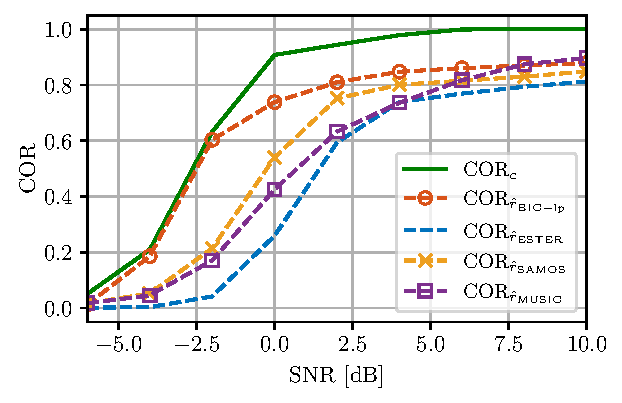
\includegraphics[width = 0.7\linewidth]{Figuras/COR_Example_random_frequencies_2.pdf}
	\caption{COR para el ejemplo de frecuencias aleatorias en función de la SNR.}
	\label{fig:COR_random}
\end{figure}
En la Fig.~\ref{fig:COR_random} se muestran las tasas de estimación de orden correcto. Para una SNR debajo de $-2$dB, la regla de selección con restricción y $BIC-lp$ tienen un rendimiento similar, que es mejor que los otros métodos. Sin embargo, cuando la SNR está por encima de $0$dB, la regla de selección con restricción presente un mejor rendimiento que los otros métodos. Para este ejemplo, VEXPA no obtuvo buenos resultados de estimación. Como se menciona en \cite{BRIANI2020}, cuando la SNR es menor a $10$dB el método VEXPA puede no devolver el orden correcto. 

\subsection{Frecuencias amortiguadas}

Se considerarán 4 ejemplos diferentes de sumas de exponenciales complejas, todas tomadas de trabajos existentes. En la tabla \ref{tab:ejemplo} se muestran los parámetros usados para la simulación numérica. En el ejemplo 1 se tiene cuatro modos: dos de esos modos se encuentran muy cerca entre sí, mientras que los otros dos están separados. El ejemplo 2 se construye añadiendo otros cinco modos al ejemplo 1, donde tres de ellos están agrupados en una región pequeña del plano complejo. En los ejemplos 3 y 4 se explora más a fondo este problema y se toma que todos  los modos están agrupados en una región del plano complejo. Esto se puede obtener cuando se muestrea un sistema de tiempo continuo usando una frecuencia alta de muestreo. Los modos ubicados en una pequeña región del plano complejo pueden ser confundidos por el método de selección de orden por un solo modo.  
\begin{table}
	\centering
	\begin{tabular}{l|lllllllll}
		& \multicolumn{9}{l}{Ejemplo 1 \cite{Andersson2014}}                                                     \\ \hline
		$\nu_i(rad^{-1})$    & 7.86   & 39.68   & 40.96   & 99.84  &         &        &        &        &        \\
		$\gamma_i(rad^{-1})$ & -0.274 & -0.150  & -0.133  & -0.221 &         &        &        &        &        \\
		$|a_i|$              & 0.4    & 1.2     & 1.0     & 0.9    &         &        &        &        &        \\
		$\angle a_i$         & -0.93  & -1.55   & -0.83   & 0.07   &         &        &        &        &        \\ \hline
		& \multicolumn{9}{l}{Ejemplo 2 \cite{Andersson2014}}                                                     \\ \hline
		$\nu_i(rad^{-1})$    & -92.16 & -7.68   & 3.71    & 11.90  & 14.98   & 19.20  & 39.68  & 40.96  & 99.84  \\
		$\gamma_i(rad^{-1})$ & -0.177 & -0.274  & -0.097  & -0.116 & -0.026  & -0.327 & -0.150 & -0.133 & -0.221 \\
		$|a_i|$              & 1.0    & 1.5     & 0.7     & 0.6    & 1.2     & 0.4    & 1.0    & 0.9    & 0.9    \\
		$\angle a_i$         & 0.42   & -0.95   & 0.40    & 0.02   & -1.55   & -0.93  & -0.83  & 0.009  & 0.007  \\ \hline
		& \multicolumn{9}{l}{Ejemplo 3 \cite{Papy2007}}                                                     \\ \hline
		$\nu_i(rad^{-1})$    & 0.2    & 0.3     & -0.2    & 0.4    & 0.35    &        &        &        &        \\
		$\gamma_i(rad^{-1})$ & -0.01  & -0.02   & -0.1    & -0.05  & -0.03   &        &        &        &        \\
		$|a_i|$              & 1.0    & 1.0     & 2.0     & 1.0    & 1.0     &        &        &        &        \\
		$\angle a_i$         & 0.0    & 0.0     & 0.0     & 0.0    & 0.0     &        &        &        &        \\ \hline
		& \multicolumn{9}{l}{Ejemplo 4 \cite{Albert2021}}                                                     \\ \hline
		$\nu_i(rad^{-1})$    & -0.22  & -0.17   & -0.026  & 0.0037 & 0.15    & 0.27   &        &        &        \\
		$\gamma_i(rad^{-1})$ & -0.01  & -0.0037 & -0.0058 & -0.012 & -0.0089 & -0.011 &        &        &        \\
		$|a_i|$              & 0.97   & 1.58    & 1.14    & 0.96   & 1.12    & 1.62   &        &        &        \\
		$\angle a_i$         & -1.78  & 2.89    & -2.46   & -1.15  & -0.32   & 0.53   &        &        &        \\ \hline
	\end{tabular}
	\caption{Parámetros usados en las simulaciones numéricas.}
	\label{tab:ejemplo}
\end{table}
Cada  modelo se prueba para diferentes niveles de potencia de ruido. Para cada modelo, y para cada SNR, se realizan $M=5000$ realizaciones independientes de \eqref{Eq:noisySignal2}. Los resultados se muestran en las figuras \ref{fig:rates} y \ref{fig:hist}. En la Fig.~\ref{fig:hist} se realizó una interpolación entre las celdas consecutivas del histograma sólo para fines de visualización. 

\begin{figure}[t]
	\begin{subfigure}[b]{0.5\linewidth}
		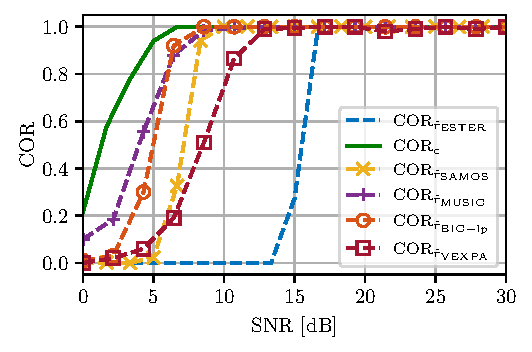
\includegraphics[width = \linewidth]{Figuras/COR_example_1_vexpa.pdf}
		\caption{Ejemplo 1}
	\end{subfigure}
	~
	\begin{subfigure}[b]{0.5\linewidth}
		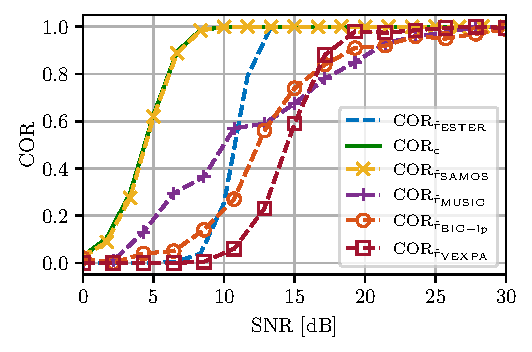
\includegraphics[width = \linewidth]{Figuras/COR_example_2_vexpa.pdf}
		\caption{Ejemplo 2}
	\end{subfigure}
	\begin{subfigure}[b]{0.5\linewidth}
		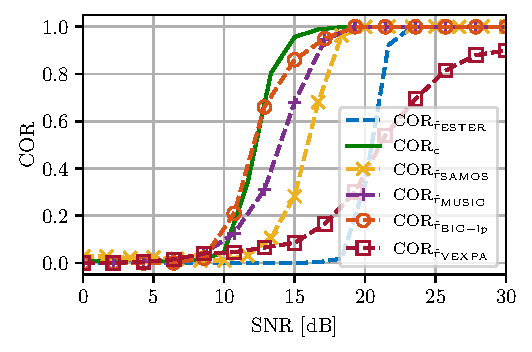
\includegraphics[width = \linewidth]{Figuras/COR_example_3_vexpa.pdf}
		\caption{Ejemplo 3}
	\end{subfigure}
	~
	\begin{subfigure}[b]{0.5\linewidth}
		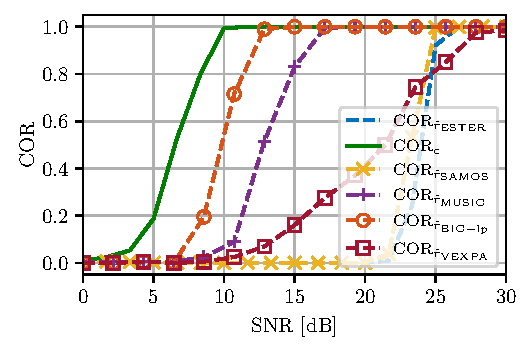
\includegraphics[width = \linewidth]{Figuras/COR_example_4_vexpa.pdf}
		\caption{Ejemplo 4}
	\end{subfigure}
	\caption{Tasa de estimación de orden correcto ($\mathrm{COR}$) en función de la SNR.}
	\label{fig:rates}
\end{figure}
\newpage
Observando la Fig.~\ref{fig:rates}, se concluye que tanto la regla ESTER como SAMOS, VEXPA y MUSIC presentan un buen desempeño cuando se tiene una alta SNR. Sin embargo, todas ellas fallan en estimar el orden correcto cuando la SNR decrece. En el caso de VEXPA, dado que se necesitan estimar las amplitudes de la señal decimada, la estimación de coeficientes de amortiguación erróneos pueden afectar la estimación. También, se puede notar que en general tanto SAMOS como MUSIC tiene un mejor desempeño que ESTER. Como se indicó en la sección \ref{sec:review} la función costo en SAMOS es el promedio del seno de todos los ángulos principales, mientras que para el ESTER la función costo sólo se tiene el seno del ángulo principal máximo.
\newpage

\begin{figure}[H]
	\centering
	\begin{subfigure}[b]{\textwidth}
		\centering
		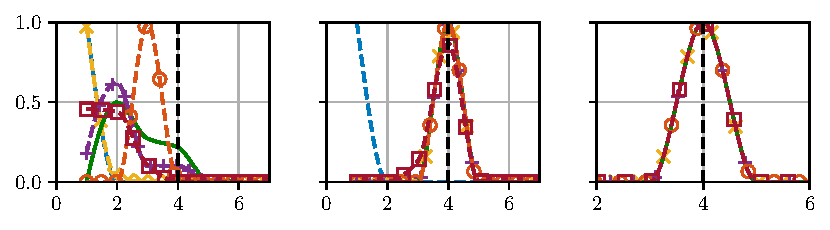
\includegraphics[width=\linewidth]{Figuras/Histogram_order_ex1_vexpa.pdf}
		\caption{Ejemplo 1}
	\end{subfigure}
	\begin{subfigure}[b]{\textwidth}
		\centering
		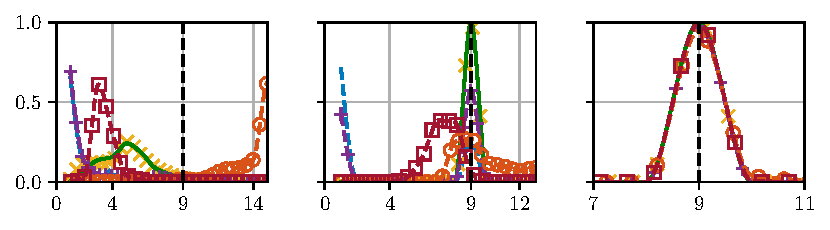
\includegraphics[width=\linewidth]{Figuras/Histogram_order_ex2_vexpa.pdf}
		\caption{Ejemplo 2}
	\end{subfigure}
	\begin{subfigure}[b]{\textwidth}
		\centering
		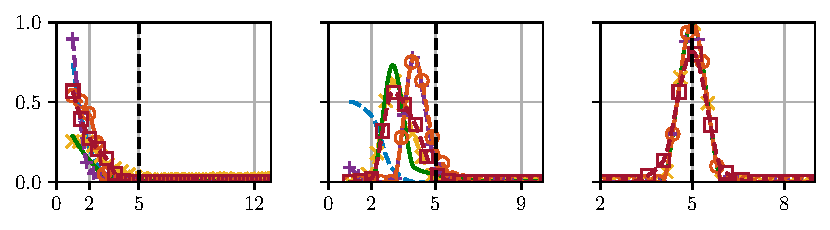
\includegraphics[width=\linewidth]{Figuras/Histogram_order_ex3_vexpa.pdf}
		\caption{Ejemplo 3}
	\end{subfigure}
	\begin{subfigure}[b]{\textwidth}
		\centering
		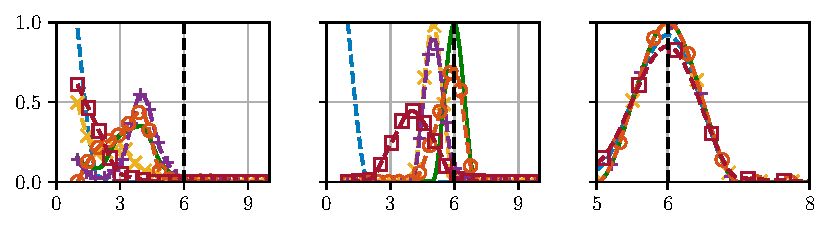
\includegraphics[width=\linewidth]{Figuras/Histogram_order_ex4_vexpa.pdf}
		\caption{Ejemplo 4}
	\end{subfigure}
	\caption{Histogrmas de los ordenes estimados: $\hat{r}_{\mathrm{ESTER}}$ en (- -)azul, $\hat{r}_{c}$ en verde, $\hat{r}_{\mathrm{BIC-lp}}$ en (-$\circ$-) rojo, $\hat{r}_{\mathrm{MUSIC}}$ en (-$+$-)Morado, $\hat{r}_{\mathrm{VEXPA}}$ en (-$\square$-) rojo oscuro, y $\hat{r}_{\mathrm{SAMOS}}$ en (-x-) amarillo. Las columnas izquierda corresponden a SNR = 0dB, las columnas del centro a SNR = 10dB, y las columnas a la derecha a SNR = 25 dB. La lineas punteadas negras indican el orden del modelo real.}	\label{fig:hist}
\end{figure}

Por otro lado, el desempeño de $\hat{r}_{\mathrm{BIC-lp}}$ se ve afectado cuando la SNR es baja. Esta última observación se explica viendo la Fig.~\ref{fig:hist} donde los histogramas muestran que la regla $\mathrm{BIC-lp}$ tiende a subestimar el orden del modelo cuando la SNR es baja. Notar que el método de selección de orden con restricción mantiene el desempeño para bajas SNR. No obstante, también recupera el desempeño de las reglas de selección basadas en métodos de subespacios. El ejemplo 4 es de particular interés para analizar el comportamiento de las reglas de selección cuando varios modos están agrupados en una pequeña región. Mientras, el método con restricción logra un buen desempeño a partir de 5 dB, ESTER y SAMOS requieren SNR por encima de los 20 dB para obtener una estimación correcta. También las reglas $\mathrm{BIC-lp}$ y MUSIC no pueden garantizar una selección de orden correcta.


\subsection{Altas SNR}\label{sec:HighSNR}

En esta sección se analizará el impacto del largo de la señal en el desempeño de las reglas de selección dado una SNR alta. En \cite{Cuyt2018} se estima el orden del modelo considerando una matriz de Hankel de $n\times n$ donde $n$ es el orden de la aproximación de Padé $R_{n-1,n}$, donde para una SNR igual a 30 dB, la brecha entre los valores singulares correspondientes al subespacio de señal y aquellos correspondientes  al subspacio de ruido se hace más notorio cuando $n\ge 500$. Para ello se considera el ejemplo presentado en \cite{Cuyt2018} y utilizado en \ref{chap:EstabilidadNumerica}. En la tabla \ref{Table:Cuyt} se muestran las frecuencias, factores de amortiguamiento y amplitudes para cada modo complejo.

\begin{table}[H]
	\centering
	\begin{tabular}{clllll}
		\multicolumn{1}{l}{Cluster} & $i$  & $\gamma_i$ & $\nu_i$      & $|c_i|$   & $\angle c_i$ \\ 
		\hline
		\multirow{6}{*}{I}            
		& 1  & -0.07      & -353.90  & 0.77   & 0.15         \\ %\cline{2-6} 
		& 2  & -0.132     & -352.02  & 6.2    & 0.0          \\ %\cline{2-6} 
		& 3  & -0.1       & -349.42  & 0.98   & 0.3          \\ %\cline{2-6} 
		& 4  & -0.11      & -348.01  & 5.4    & 0.9          \\ %\cline{2-6} 
		& 5  & -0.12      & -347.01  & 6.1    & 0.7          \\ %\cline{2-6} 
		& 6  & -0.081     & -345.00  & 0.95   & 0.2          \\ 
		\hline
		\multirow{5}{*}{II}          
		& 7  & -0.106     & -132.50  & 4.71   & 0.12         \\ %\cline{2-6} 
		& 8  & -0.129     & -131.40  & 3.9    & 0.1          \\ %\cline{2-6} 
		& 9  & -0.203     & -130.01  & 7.0    & -0.234       \\ %\cline{2-6} 
		& 10 & -0.16      & -129.17  & 5.43   & 0.2          \\ %\cline{2-6} 
		& 11 & -0.19      & -128.09  & 4.4    & -0.52        \\ 
		\hline 
		\multirow{2}{*}{III}          
		& 12 & -0.102     & 14.10    & 3      & 0.21         \\ %\cline{2-6} 
		& 13 & -0.127     & 15.81    & 3      & -0.8         \\ %\hline \hline
		\hline 
		\multirow{7}{*}{IV}           
		& 14 & -0.076     & 107.70   & 0.39   & -0.3         \\ %\cline{2-6} 
		& 15 & -0.091     & 110.24   & 0.37   & -0.8         \\ %\cline{2-6} 
		& 16 & -0.1       & 112.50   & 0.36   & 0.1          \\ %\cline{2-6} 
		& 17 & -0.08      & 114.00   & 0.3    & 0.9          \\ %\cline{2-6}
		%\multirow{3}{*}{V}            
		& 18 & -0.21      & 124.01  & 3.2    & -0.106       \\ %\cline{2-6} 
		& 19 & -0.15      & 125.62  & 5.53   & 0.2          \\ %\cline{2-6} 
		& 20 & -0.173     & 126.98  & 4.7    & -0.3         \\ %\hline \hline
		\hline 
		\multirow{5}{*}{V}           
		& 21 & -0.11      & 434.00  & 1      & -0.15        \\ %\cline{2-6} 
		& 22 & -0.12      & 435.38  & 5      & 0.26         \\ %\cline{2-6} 
		& 23 & -0.157     & 436.19  & 6.1    & -0.2         \\ %\cline{2-6} 
		& 24 & -0.12      & 437.97  & 5.1    & 0.0          \\ %\cline{2-6} 
		& 25 & -0.18      & 439.51  & 6      & -0.1         \\ %\hline
		\hline 
	\end{tabular}
	\caption{La señal contiene 25 modos complejos agrupados en $5$ regiones}.\label{Table:Cuyt}
\end{table}			
			

\begin{figure}[h!]
	\centering
	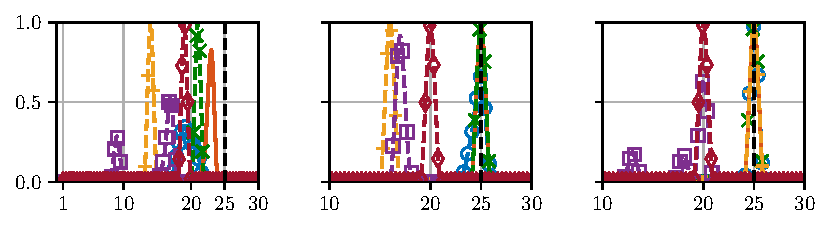
\includegraphics[width=\linewidth]{Figuras/Histogram_order_cuyt_vexpa.pdf}
	\caption{Histograma del orden estimado para $SNR = 30dB$. $\hat{r}_{\mathrm{VEXPA}}$($-\circ-$); $\hat{r}_c$ ($-$); $\hat{r}_{\mathrm{ESTER}}$ ($-\times-$); $\hat{r}_{\mathrm{SAMOS}}$ ($-+-$); $\hat{r}_{\mathrm{MUSIC}}$ ($-\square-$); $\hat{r}_{\mathrm{BIC-lp}}$ ($-\diamond-$). Las columnas izquierda corresponden a $n=400$, las columnas del centro a $n=500$, y las columnas a la derecha a $n=600$. La lineas punteadas negras indican el orden del modelo real.}
	\label{Fig:cuyt}
\end{figure}
El Histograma de los órdenes estimado se muestra en la Fig.~\ref{Fig:cuyt} para $n=400,500,600$. Se puede ver que para $n=400$, todos los métodos obtienen estimaciones incorrectas. Sin embargo, cuando $n\ge 500$ la regla de optimización propuesta, como también ESTER y VEXPA, estiman el orden correcto, mientras los otros métodos siguen obteniendo órdenes incorrectos. SAMOS necesita al menos  $n=600$ para mejor su desempeño. Previamente, se mencionó que para altas SNR los métodos basados en el teorema de Kronecker presentan un buen desempeño. Sin embargo, esto es cierto cuando la longitud de la señal es lo suficientemente grande. En este ejemplo, se observa que el problema de optimización propuesto en \eqref{eq:propuesta3} logra un buen rendimiento, incluso cuando la longitud de la señal es pequeña.

\subsection{Ruido Coloreado}

Se considerará un ejemplo donde la señal está perturbada por ruido coloreado. Para ello, una secuencia de ruido blanco $w_k\sim\NormalC(0,1)$ se filtrará produciendo una secuencia de ruido coloreado $u_k$. Considerando el Lema \ref{Lemma:2} se tiene que 

\begin{equation}
	\|\Hank_{\u}\|_2\le \max_k |\e_k^T\matV\u|\le \max_k |H_k|\max_k|\e_k^T\matV\w|
	\label{Eq:normHu}               
\end{equation}
donde $\matV$ es la matriz de DFT, $|H_k|$ son muestras en el dominio de la frecuencia del filtro de coloreado. Luego, por el Teorema \ref{Th:boundHankelMatrix2} se obtiene la siguiente cota
\begin{equation}
	\tau = \max_k|H_k|\sqrt{-(2n-1)\log(1-\beta^{\frac{1}{2n-1}})}.
	\label{Eq:bound}
\end{equation}

A continuación se comparará el desempeño de todos los métodos de estimación de orden vistos anteriormente cuando se tiene ruido coloreado. Se utiliza el Ejemplo 1 en la Tabla \ref{tab:ejemplo}. El ruido coloreado se obtiene, aplicando el filtro
 \[H(e^{\jmath\omega}) = \frac{\eta}{1+ae^{-\jmath\omega}}\] a un vector de ruido blanco $\w\sim\mathcal{CN}(\mathbf{0},\matI_{2n-1})$, donde $\eta$ se ha elegido de manera de obtener una SNR resultante de 10 dB. En la Figura \ref{Fig:colored_noise} se muestran los histogramas de los órdenes estimados para $a=-0.6,-0.7,-0.8$. Se puede observar que para el caso de $a=-0.6$ tanto la regla de optimización propuesta en este trabajo como SAMOS logran estimar el orden del modelo correcto, mientras que los otros métodos tiene un peor desempeño. A medida que $|a|\to 1$ el desempeño de todos los métodos se ve deteriorado. Sin embargo, el método de optimización presenta el mejor desempeño entre todos los otros métodos.

\begin{figure}[H]
	\centering
	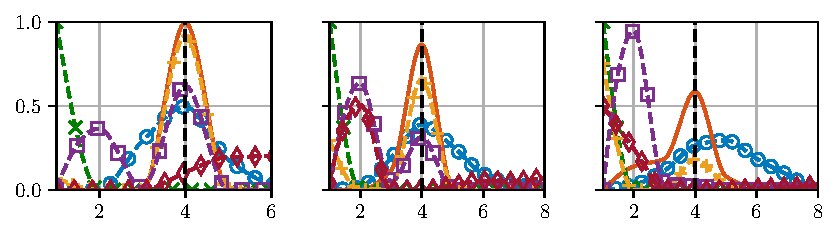
\includegraphics[width=\linewidth]{Figuras/Histogram_order_coloredNosie_vexpa.pdf}
	\caption{Histograma del orden estimado para $SNR = 10dB$. $\hat{r}_{\mathrm{VEXPA}}$($-\circ-$); $\hat{r}_c$ ($-$); $\hat{r}_{\mathrm{ESTER}}$ ($-\times-$); $\hat{r}_{\mathrm{SAMOS}}$ ($-+-$); $\hat{r}_{\mathrm{MUSIC}}$ ($-\square-$); $\hat{r}_{\mathrm{BIC-lp}}$ ($-\diamond-$). La columna izquierda corresponde a $a=-0.6$, centro a $a = -0.7$, y la derecha a $a=-0.8$. La lineas punteadas negras indican el orden del modelo real.}
	\label{Fig:colored_noise}
\end{figure}

%\section{Conclusiones}\label{sec:Conclusiones}

%En este capítulo, se consideró el problema de la selección del orden del modelo para señales compuestas por una suma de exponenciales complejas. La nueva propuesta explota la propiedad de invariancia de la matriz de Hankel, que es beneficiosa cuando existe una buena separación entre el ruido y el subespacio de la señal. Sin embargo, también impone una restricción sobre los valores singulares de la matriz de Hankel observada para penalizar las estimaciones de orden pequeño cuando la SNR es baja. Al resolver un problema de optimización con restricciones, el objetivo es resolver ambos problemas simultáneamente: descartar los componentes ruidosos de la señal y preservar la estructura de la señal. La restricción del problema de optimización se construye acotando superiormente la norma espectral de la matriz de Hankel asociada a la señal contaminada con ruido. En particular, cuando el ruido es Gaussiano, obtenemos una expresión analítica para su función de distribución. Usando aproximaciones numéricas, también se obtuvieron límites apropiados cuando se desconoce el nivel de potencia del ruido. Para probar el rendimiento del esquema propuesto, se han comparado con reglas de selección previamente conocidas usando ejemplos que ya publicados. Tomando varios ejemplos de sumas exponenciales de diferentes órdenes con frecuencias aleatorias no amortiguadas y frecuencias amortiguadas que podrían estar muy agrupadas muy cerca entre sí. Cada ejemplo se testeó con diferentes valores de SNR. En todos los casos, esta nueva propuesta mostró el mejor rendimiento para una amplia gama de valores de SNR.

%\newpage
\section{Apéndice}
%\addcontentsline{toc}{section}{\bfseries Appendices}
%\renewcommand{\thesubsection}{\arabic{subsection}}
%\setcounter{subsection}{0}
\subsection{Tabla de los parámetros usados en VEXPA}\label{appex:Vexpa}

Parámetros usados por el algoritmo VEXPA en las simulaciones de los distintos ejemplos del capítulo
\begin{table}[h!]
	%\centering
	\hspace{-1cm}
	\begin{tabular}{c|ccccccc}
		& u & s & $\delta_u$ & $\delta_s$ & $m_u$ & $m_s$ & m  \\ 
		ejemplo 1 & 4 & 3 & 0.1        & 0.1        &  3    & 3     & 8 \\
		ejemplo 2 & 5 & 11 & 0.1 & 0.1 & 4 & 3 & 20\\
		ejemplo 3 & 3 & 2 & 0.1 & 0.1 & 3 & 3 & 10\\
		ejemplo 4 & 6 & 5 & 0.1 & 0.1 & 4 & 3 & 20\\
		ejemplo en secc. \ref{sec:HighSNR} & 5 & 11 & $[0.01,0.03,0.05]$ & $[0.01,0.03,0.05]$ & $[5,4,3]$ & $[5,4,3]$ & 35\\
	\end{tabular}
	\caption{Parámetros usados en VEXPA}
	\label{tab:vexpa_parameters}
\end{table}
